\documentclass{article}

\usepackage{times}
\usepackage{amssymb, amsmath, amsthm}
\usepackage[margin=.5in]{geometry}
\usepackage{graphicx}
\usepackage[linewidth=1pt]{mdframed}

\usepackage{import}
\usepackage{xifthen}
\usepackage{pdfpages}
\usepackage{transparent}
\usepackage{float}

\newcommand{\incfig}[1]{%
    \def\svgwidth{\columnwidth}
    \import{./figures/}{#1.pdf_tex}
}

\newtheorem{theorem}{Theorem}[section]
\newtheorem{lemma}{Lemma}[section]
\newtheorem*{remark}{Remark}
\theoremstyle{definition}
\newtheorem{definition}{Definition}[section]

\begin{document}

\title{General Relativity - Homework 6}
\author{Philip Warton}
\date{\today}
\maketitle
\section*{Problem 1}
\subsection*{a)}
We must manipulate our function algebraically as follows,
\begin{align*}
  8mr &= h^2 + 16m^2 \\
  8mr - 16m^2 &= h^2 \\
  \pm\sqrt{8mr - 16m^2} &= h
\end{align*}
Plotting this function with $m$ fixed to be some constant (in our case $m=1$, but the overall shape
is invariant), we get
\begin{figure}[H]
    \centering
    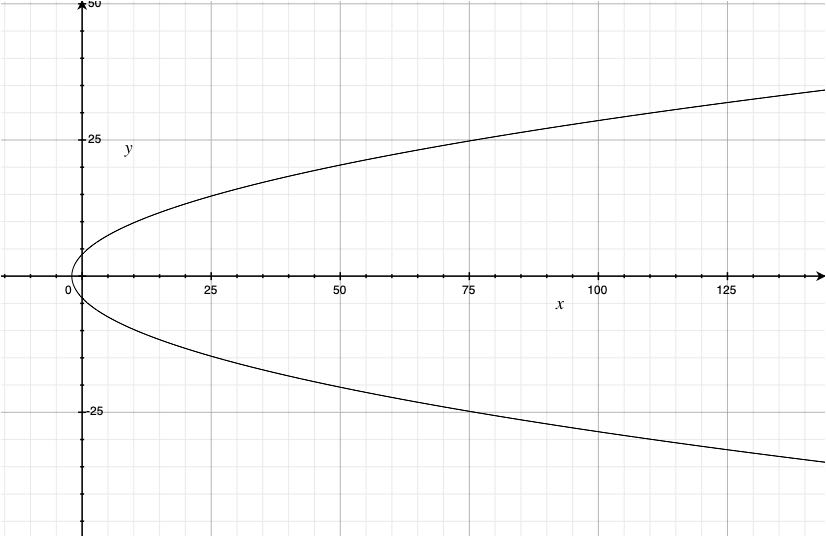
\includegraphics[width=10cm]{figures/1.jpg}
    \caption{$h = \pm\sqrt{8mr - 16m^2}$}
  \end{figure}
\subsection*{b)}
To compute the arclength in terms of $r$ and $dr$, we wish to use the Euclidean line element.
We say that 
\[
  ds^2 = dr^2 + dh^2
\]
We must take the derivative of $h$ with respect to $r$.
\[
  \frac{d}{dr}\left(\pm\sqrt{8mr-16m^2}\right) = \frac{\pm 8m}{2\sqrt{8mr-16m^2}}
\]
Then we want to use this to compute our arclength.

\begin{align*}
  L &= \int_a^b \sqrt{1 + f'^2(r)}dr \\
  &= \int_a^b \sqrt{1 + \left(\frac{\pm8m}{2\sqrt{8mr-16m^2}}\right)^2} dr \\
  &= \int_a^b \sqrt{1 + \frac{2m^2}{mr-2m^2}} dr \\
  &= \int_a^b \sqrt{\frac{mr}{mr-2m^2}}dr \\
  &= \int_a^b \sqrt{\frac{r}{r-2m}}dr \\
  &= \int_a^b \frac{dr}{\sqrt{1- \frac{2m}{r}}}
\end{align*}
And we say that this is the arclength of our parabola based on $a,b$ and $m$. However,
we notice that this term within the integral looks highly similar to $\sigma^r$ from Schwarzchild geometry.
\subsection*{c)}
To rotate around the $h$-axis, consider a new coordinate, $\phi$. If we 
take our line element, and write $dh$ in terms of $r$ and $dr$ we may be able to more 
easily understand the geometry of what we are doing.
Since $h = \pm \sqrt{8mr - 16m^2}$ we can write 
\begin{align*}
  h & = \sqrt{8mr - 16m^2} \\
  dh &= d\left( \sqrt{8mr - 16m^2} \right) \\
  &= 0 \cdot dm + \frac{dr}{\sqrt{\frac{r}{2m} - 1}}
\end{align*}
Then our line element becomes
\begin{align*}
  ds^2 &= dr^2 + dh^2 \\
  &= dr^2 +  \left(\frac{dr}{\sqrt{\frac{r}{2m} - 1}}\right)^2 \\
  &= dr^2\left(1 + \frac{1}{\frac{r}{2m} - 1}\right)\\
  &= dr^2 \left(\frac{\frac{r}{2m} - 1 + 1}{\frac{r}{2m}-1}\right)\\
  &= dr^2\left(\frac{\frac{r}{2m}}{\frac{r}{2m}-1}\right)\\
  &=dr^2\left(\frac{1}{1-\frac{2m}{r}}\right)\\
  &=\frac{dr^2}{1-\frac{2m}{r}}
\end{align*}
Knowing that if we fix some radius, are arclength traveling along $\phi$ should mimic
a circular arclength (given that we are rotating our whole parabola in a circle), we add
a $\phi$ piece to our line element yielding
\[
  ds^2 = \frac{dr^2}{1- \frac{2m}{r}} + r^2d\phi
\]
Then if $dr = 0$ and we have a fixed radius, we should get arclength that is equal to a circle.
Notice that this is equal to the line element of the Schwarzchild geometry given that $dt = 0$ and 
that $\theta = \frac{\pi}{2}$.
\subsection*{d)}
Given our line element $ds^2$ we say that our basis forms are given by 
\begin{align*}
  \sigma^r &= \frac{dr}{\sqrt{1- \frac{2m}{r}}}\\
  \sigma^\phi &= rd\phi
\end{align*}
So then by the torsion free condition we say that
\begin{align*}
  0 &= d\sigma^r + \omega^r_{\ \phi} \wedge \sigma^\phi\\
  0 &= d\left(\frac{dr}{\sqrt{1-\frac{2m}{r}}}\right) + \omega^r_{\ \phi} \wedge rd\phi\\
  0 & = \omega^r_{\ \phi} \wedge r d\phi
\end{align*}
By the torsion free condition we say that 
\begin{align*}
  0&= d\sigma^\phi + \omega^\phi_{\ r} \wedge \sigma^r \\
  0 &= d(rd\phi) + \omega^\phi_{\ r} \wedge \left(\frac{dr}{\sqrt{1- \frac{2m}{r}}}\right)\\
  0 &= dr \wedge d\phi  + r \wedge d^2 \phi + \omega^\phi_{\ r} \wedge \left(\frac{dr}{\sqrt{1- \frac{2m}{r}}}\right) \\
  0 &= dr \wedge d\phi + \omega^\phi_{\ r} \wedge \left(\frac{dr}{\sqrt{1- \frac{2m}{r}}}\right)\\
  0 &= \sqrt{1 - \frac{2m}{r}}dr \wedge d\phi + \omega^\phi_{\ r} \wedge dr \\
  \sqrt{1-\frac{2m}{r}}d\phi \wedge dr &= \omega^\phi_{\ r} \wedge dr\\
  \sqrt{1-\frac{2m}{r}}d\phi & = \omega^\phi_{\ r}
\end{align*}
Then by metric compatibility we say that $\omega^r_{\ \phi} = -\sqrt{1 - \frac{2m}{r}}d\phi$.
Finally we can write 
\begin{align*}
  \Omega^r_{\ \phi} &= d \omega^r_{\ \phi} = K\omega \\
  &= d\left(-\sqrt{1-\frac{2m}{r}}d\phi\right) \\
  K \omega &= \frac{-m}{r^2}\cdot \frac{1}{\sqrt{1- \frac{2m}{r}}}dr \wedge d\phi
\end{align*}
Then since $\omega$ is our orientation which given the line element can be written \[
  \omega = \frac{dr}{\sqrt{1-\frac{2m}{r}}} \wedge rd\phi
\]
We write that 
\begin{align*}
  K\left(\frac{dr}{\sqrt{1-\frac{2m}{r}}} \wedge rd\phi\right) & = \frac{-m}{r^2}\cdot \frac{1}{\sqrt{1- \frac{2m}{r}}}dr \wedge d\phi \\
  K\left(\frac{r}{\sqrt{1-\frac{2m}{r}}}\right)dr \wedge d\phi &= \frac{-m}{r^2}\cdot \frac{1}{\sqrt{1- \frac{2m}{r}}}dr \wedge d\phi \\
  K\left(\frac{r}{\sqrt{1-\frac{2m}{r}}}\right) &= \frac{-m}{r^2}\cdot \frac{1}{\sqrt{1- \frac{2m}{r}}} \\
  Kr &= \frac{-m}{r^2}\\
  K &= \frac{-m}{r^3}
\end{align*}
And we say that this is the curvature of our surface devised in \fbox{1c}.
\section*{Problem 2}
\subsection*{a)}
We seek to describe $\vec e_i \cdot \vec \nabla f$ in terms of partial derivatives.
Now we can say that 
\begin{align*}
  \vec e_i \cdot \vec \nabla f & = \vec e_i \cdot \begin{pmatrix}
    \frac{\partial}{\partial x_1}\vec e_1 \\
    \vdots \\
    \frac{\partial}{\partial x_n}\vec e_n
  \end{pmatrix}\\
  &= \sum_{j = 1}^n \frac{\partial}{\partial x_j}\vec e_i \cdot \vec e_j \\
  &= \sum_{j=1}^n \frac{\partial}{\partial x_j}g_{ij}
\end{align*}
Which is the sum of the Jacobian $J_g$ where $g$ is the metric on the $i$-th row.
\subsection*{b)}
We wish to express $g^{ij} = g(dx^i,dx^j)$ in terms of of components $g_{ij}$.
Let $\vec u_i$ be a vector such that $\vec u_i \cdot d\vec{r} = dx^i$.
This vector must exist by definition of our basis forms.
Now we get the following system of equations
\begin{align*}
  dx^i & = \sum_{j = 1}^n dx^j(\vec u_i \cdot \vec e_j)
  \begin{pmatrix}
    dx^1\\
    \vdots\\
    dx^n
  \end{pmatrix}\\
   & = \begin{pmatrix}
    \sum_{j = 1}^n dx^j(\vec u_1 \cdot \vec e_j)\\
    \vdots\\
    \sum_{j = 1}^n dx^j(\vec u_n \cdot \vec e_j)
  \end{pmatrix}\\
  &= \begin{pmatrix}
    \vec u_1 \\
    \vdots \\
    \vec u_n
  \end{pmatrix}
  \cdot \begin{pmatrix}
    dx^1 \vec e_1 \\
    \vdots \\
    dx^n \vec e_n
  \end{pmatrix}
\end{align*}
We know that along the diagonal of $g$ we will get 1's, and elsewhere we will get 0's,
given we have an orthonormal basis, so it follows that $g^{ij} = g(dx^i, dx^j) = \vec u_i \cdot \vec u_j$.
Thus we have 
\[
  \sum_{j = 1}^n g^{ij}g_{jk} = \delta^i_{\ k}
\]
Where $\delta^i_{\ j} = \begin{cases}
  1 & i = j \\
  0 & i \neq j
\end{cases}$. So it follows that we can write this as a matrix product 
\[
  g^\circ \times g_\circ = I
\]
And it follows that $g_{ij}$ works as the corresponding element to the inverse matrix of $g^{ij}$.
\end{document}